\chapter{More on fitting}

%%%%%%%%%%%%%%%%%%%%%%%%%%%%%%%%%%%%%%%%%%%%%%%%%%%%%%%%%%%%%%%%%%%%%%%%%%%%%%%%
\section{Gentle introduction to data fitting}
  \SecLabel{FittingGentleIntroducion}
%%%%%%%%%%%%%%%%%%%%%%%%%%%%%%%%%%%%%%%%%%%%%%%%%%%%%%%%%%%%%%%%%%%%%%%%%%%%%%%%

The aim of this section is to briefly introduce the basic concepts of
data fitting, its key terminology and difficulties which might arise
when fitting scattering data.
Users wanting to find out more about minimization (also called
maximization or optimization methods depending on the formulations and objectives) 
or looking for more detailed discussions are referred to \cite{AnLu07, mntutorial}

\subsection{Toy scattering experiment}

Figure~\ref{fig:toyfit_data},left shows a scattering intensity map in arbitrary units  
as a function of $(x,y)$, the positions on the detector ``measured'' in this toy scattering experiment.

\begin{figure}[!p]
  \centering
    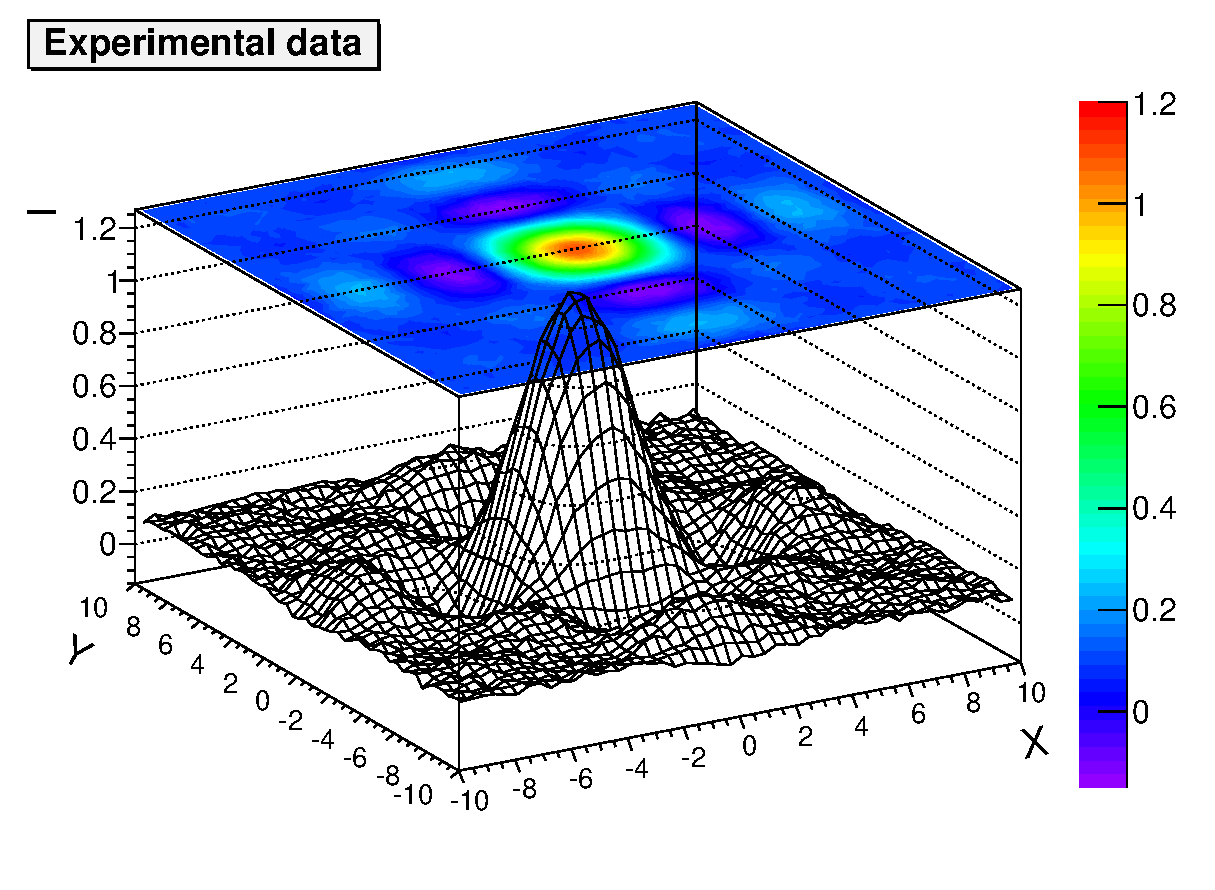
\includegraphics[width=0.49\textwidth]{fig/unused/toyfit_expdata.eps}
    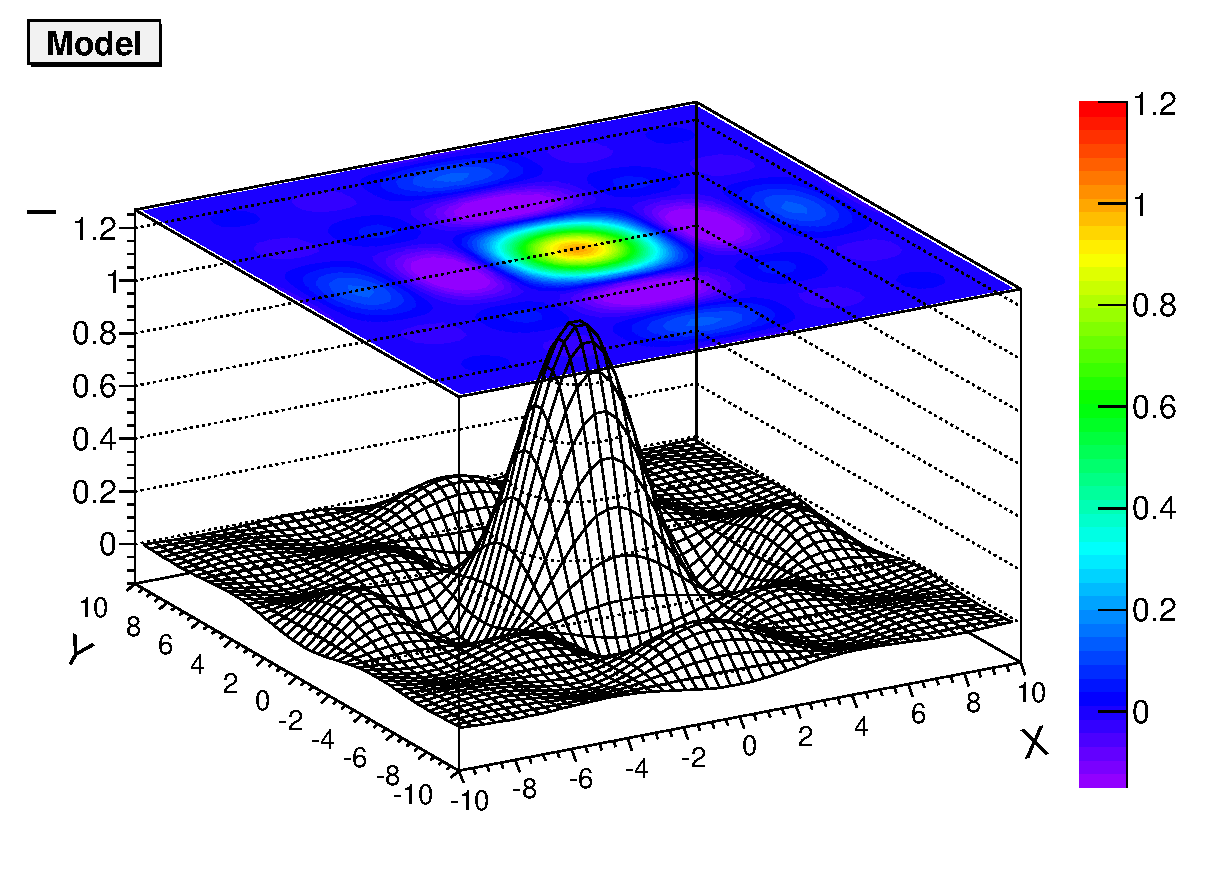
\includegraphics[width=0.49\textwidth]{fig/unused/toyfit_simdata.eps}
  \caption{Intensity as a function of (x,y) detector coordinates  obtained from 
  toy experiment (left) and from the toy simulation (right).   }
  \label{fig:toyfit_data}
  \vspace*{4mm}
    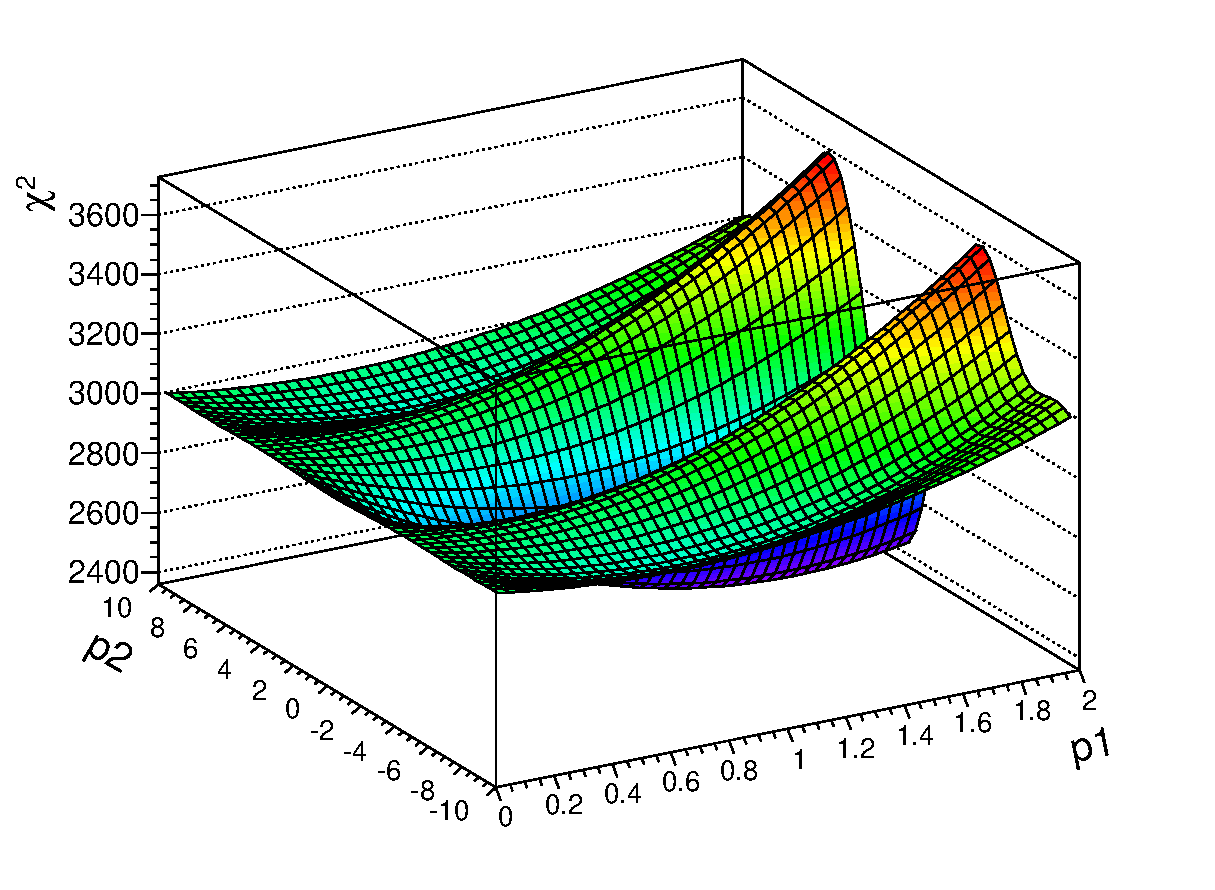
\includegraphics[width=0.49\textwidth]{fig/unused/toyfit_chi2_p12.eps}
    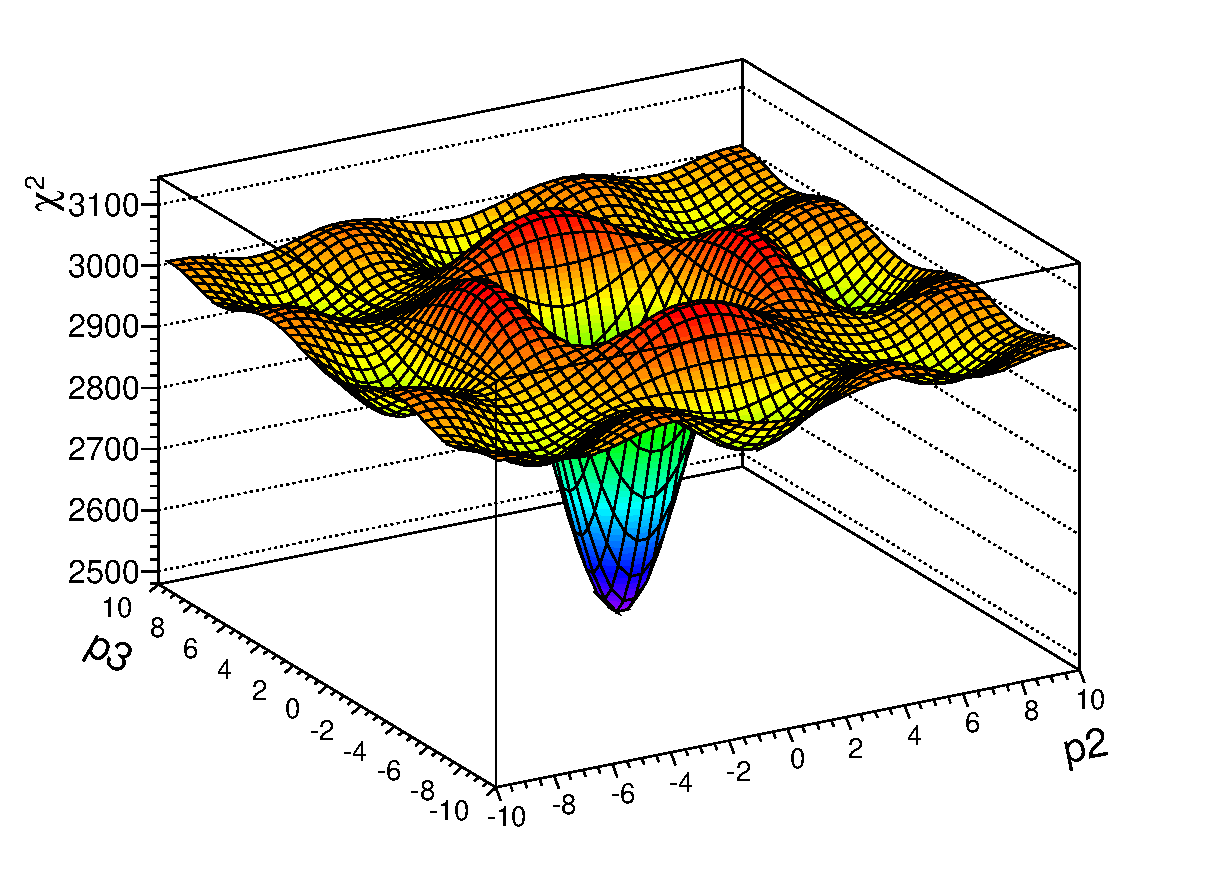
\includegraphics[width=0.49\textwidth]{fig/unused/toyfit_chi2_p23.eps}
  \caption{$\chi^{2}$ value calculated between experimental and simulated data
  as a function of $p_1,p_2$ parameters (left) or $p_2,p_3$ 
  parameters (right) used in the model.   }
  \label{fig:toyfit_chi2}
\end{figure}


The scattering picture, similar to some GISAS patterns, has been generated using the simple function
$$I(x,y) = G(0.1,~0.01) + sincx(x) \cdot sinc(y)$$
Here $G(0.1, 0.01)$ is a random variable distributed according to a Gaussian distribution
with a mean of 0.1 and a standard deviation $\sigma=0.01$.
Constant $0.1$ symbolizes our experimental background and constant $0.01$ refers
to the detector noise. The rest of the formula represents our signal.

Let's define our model, namely specific mathematical functions, to
which we will fit our toy experimental data. By making an educated
guess we assume that the scattering intensity observed
in the experiment should be described by $sinc$ functions as follows
\begin{equation} \label{eq:toy_model}
f(x,y;p) = p_0 + p_1 \cdot  sinc(x - p_2) \cdot sinc(y - p_3)
\end{equation}

The model has four parameters: $p_0$ describes a constant background,
$p_{1}$ describes the signal strength
and $p_2,p_3$ give the peak position along the $x$ and $y$ axis, respectively.
Figure~\ref{fig:toyfit_data},right shows the intensity as a function
of $(x,y)$ calculated using  our model and a fixed set of parameters 
$p_0=0, p_1=1, p_2=0, p_3=0$. 

The two distributions are qualitatively identical. However in order to find the
values of parameters which best describe the experimental data, one has to
\begin{itemize}
\item define criteria for the difference between the actual data and the model,
\item use a minimization procedure, which will minimize this difference.
\end{itemize}


\subsection{Objectives}

The goal is to obtain the best fit of an observed distribution
to a prediction by modifying a set of parameters from this
prediction. This problem can be one or multi-dimensional and also linear or
nonlinear. The quantity to minimize is often referred to as the
\textit{objective function}, whose expression depends on the
particular method, like the maximum likelihood, the $\chi^2$
minimization or the expected prediction error function. 

\begin{comment}
\subsubsection*{Maximum of likelihood}
This is a popular method for parameters' estimations because the maximum likelihood estimators are approximately
unbiased and efficient for large data samples, under quite general
conditions.
We assume a sample  $\mathbf{x}=\{x_{1},x_{2},...,x_{n}\}$ of n independent and identically distributed
observations coming from probability density function $f(\mathbf{x}; \mathbf{p})$.
We assume $f(\mathbf{x}; \mathbf{p})$
to be known except for the parameters $\mathbf{p}=\{p_1,p_2,...,p_3\}$
The method of maximum likelihood takes the estimators to be
those values of $\mathbf{p}$ that maximize the likelihood function $\mathcal{L}$ as
$\mathcal{L}(\mathbf{\alpha})=\prod_{i=1}^N f(x_i;\mathbf{p})$.
Since it is easier to deal with a sum, we usually minimize
$-\text{ln}(\mathcal{L})$.
\end{comment}


\subsubsection*{$\chi^2$ or least squares minimization}
Performing $N$ measurements generates $N$ pairs of data $(\mathbf{x_{i}}, a_{i}), i=1,N$ where 
$\mathbf{x_{i}}$ is an independent variable and $a_{i}$ is a dependent variable, whose
value is found during measurement $i$.

In the case of the intensity map measured in our toy experiment 
and presented in Fig~\ref{fig:toyfit_data}, variable $a_{i}$ denotes
the measured intensity, variable $\mathbf{x_{i}}$ is a vector and
corresponds to the pixel coordinates $(x_{i}, y_{i})$ in our detector while $N$ corresponds 
to total number of detector pixels.

The model function has the form
$f(\mathbf{x_{i}},\mathbf{p})$
where adjustable parameters are held in vector $\mathbf{p}$.
The least squares method finds the optimum of the model function by searching the minimum of the sum of squared
residuals
$$ \chi^{2}(\mathbf{p}) = \sum_{i=1}^{N}r_{i}^{2}$$
where the residual is defined as the difference between the measured value and the value predicted by the model.
$$r = a_{i} - f(\mathbf{x_{i}},\mathbf{p})$$

In case of normally distributed variables with a variance $\sigma^2$,
the quantity to minimize becomes
$$ \chi^{2}(\mathbf{p}) =
\frac{1}{d}
\sum_{i=1}^{N}  
\frac{ (a_{i} - f(\mathbf{x_{i}},\mathbf{p}))^2}{\sigma^2}   $$
where $d=N-k$ is number of degree of freedom ($k$ being the number of free fit parameters).

\subsubsection*{Maximum of likelihood}
to be written


\subsubsection*{Minimization algorithms}
There is a large number of algorithms to minimize the objective function over the space of parameters of the function.
The minimization starts from an initial guess for the parameters
provided by the user. Then the process evolves iteratively under the
control of the minimization algorithm. The procedural
modifications on the parameters, the objective function, as well as
the convergence
criteria depend on the method implemented.
Details of all implementations are beyond the scope of this manual.



\subsubsection*{Local minima trap}
Finding the global minimum of the objective function 
is a general problem in optimization that is unlikely to have an exact and 
tractable solution. This issue can be illustrated using our toy experiment.

The theoretical model given by formula \ref{eq:toy_model} is defined
in $(x,y)$ space and additionally depends on parameter vector $\mathbf{p}$. 
The $\chi^2$ 
objective function is obtained by calculating the sum of squared residuals between
the measured (Fig.~\ref{fig:toyfit_data}, left) and the 
predicted (Fig.~\ref{fig:toyfit_data}, right) values over $x,y$ space. It is defined
in parameter space $\mathbf{p}$, which has 4 dimensions.

Figure~\ref{fig:toyfit_chi2} (left) shows the $\chi^2$ distribution as a function of
parameters $p_1,p_2$  while parameters $p_0,p_3$ remain fixed.
Figure~\ref{fig:toyfit_chi2} (right) shows the $\chi^2$ distribution as a function of
parameters $p_2,p_3$ while parameters $p_0,p_1$ remain fixed.

One can see that the given objective function has a strongly
pronounced global minimum, which we aim to determine. In addition the
objective function presents a number of local minima.
The presence of these minima leads to slow, or even no convergence
towards the  single global minimum.


\subsection{Terminology}

\noindent
{\bf Reference data} \\
In general they are just experimental data or they might be also simulated data
perturbed  with some noise for the purpose of testing minimization algorithms.
\vspace*{1mm}

\noindent
{\bf Objective function} \\
Subject of the minimization procedure.
\vspace*{1mm}

\noindent
{\bf Minimization} \\
Finding the best available values (i.e. local minimum) of some objective function. 
\vspace*{1mm}

\noindent
{\bf Number of degrees of freedom} \\
Number of data points - number of parameters in the fit.
\vspace*{1mm}

\noindent
{\bf Minimizer} \\
Algorithm which minimizes the objective function. 

